\chapter{Background}
\label{sec:background}

In the first part of the thesis we look at the current state of configuration file parsing according to the literature. After that we provide a short overview of Elektra, the key-value storage framework we use in the thesis. At the end of this chapter we provide some examples of other research papers that evaluate parsers and parser engines.

\section{State of the Art}
\label{sec:state_of_the_art}

\subsection{Parsing}
\label{sec:parsing}

The book \citetitle{grune2008parsing}~\cite{grune2008parsing} provides a good overview of various up-to-date parsing algorithms. It covers the most popular techniques and also less well known methods up to 2006. The book also describes various classification possibilities for parsing techniques \cite[p. 85]{grune2008parsing}. The most common classification is the division into bottom-up and top-down parsers.

\begin{figure}
  \centering
  \begin{subfigure}[t]{.48\textwidth}
    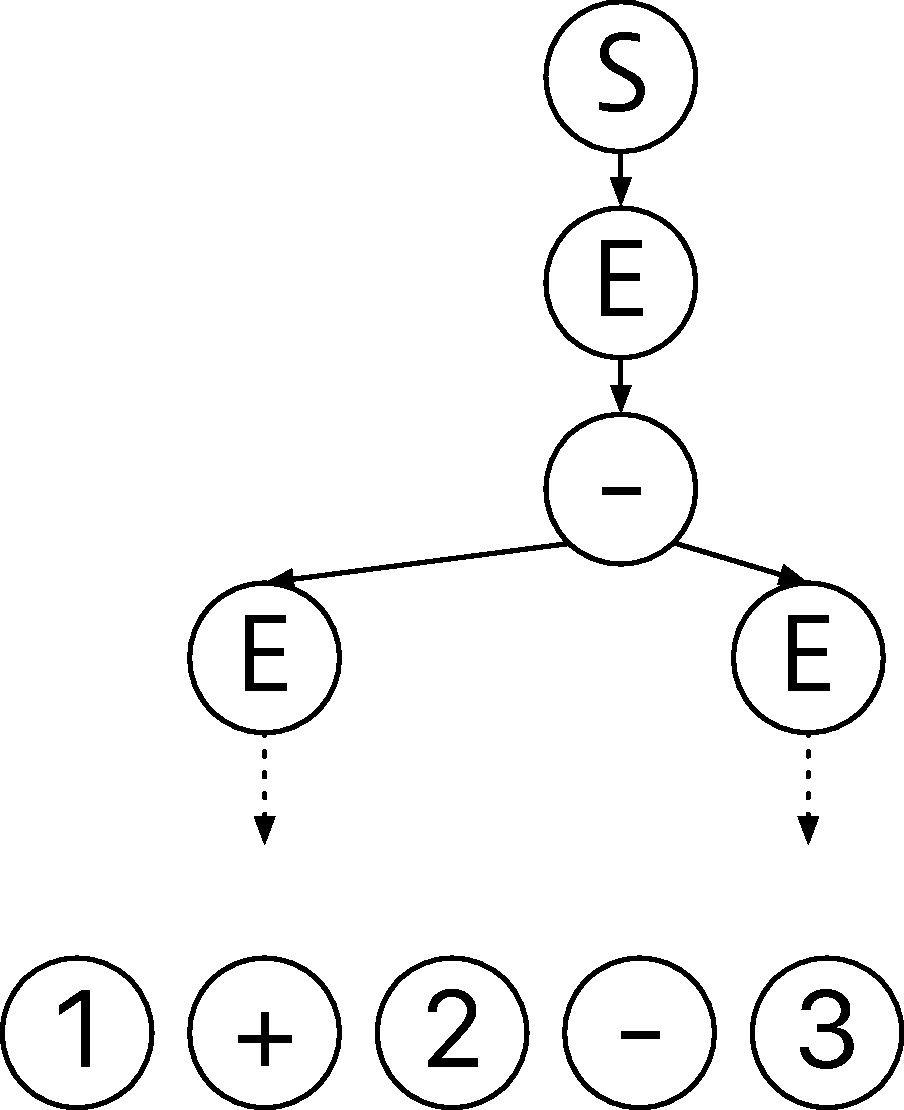
\includegraphics[width=\linewidth]{Top-Down}
    \caption{A top-down parser predicts and matches rules from the start symbol downwards.}
  \end{subfigure}
  \quad
  \begin{subfigure}[t]{.48\textwidth}
    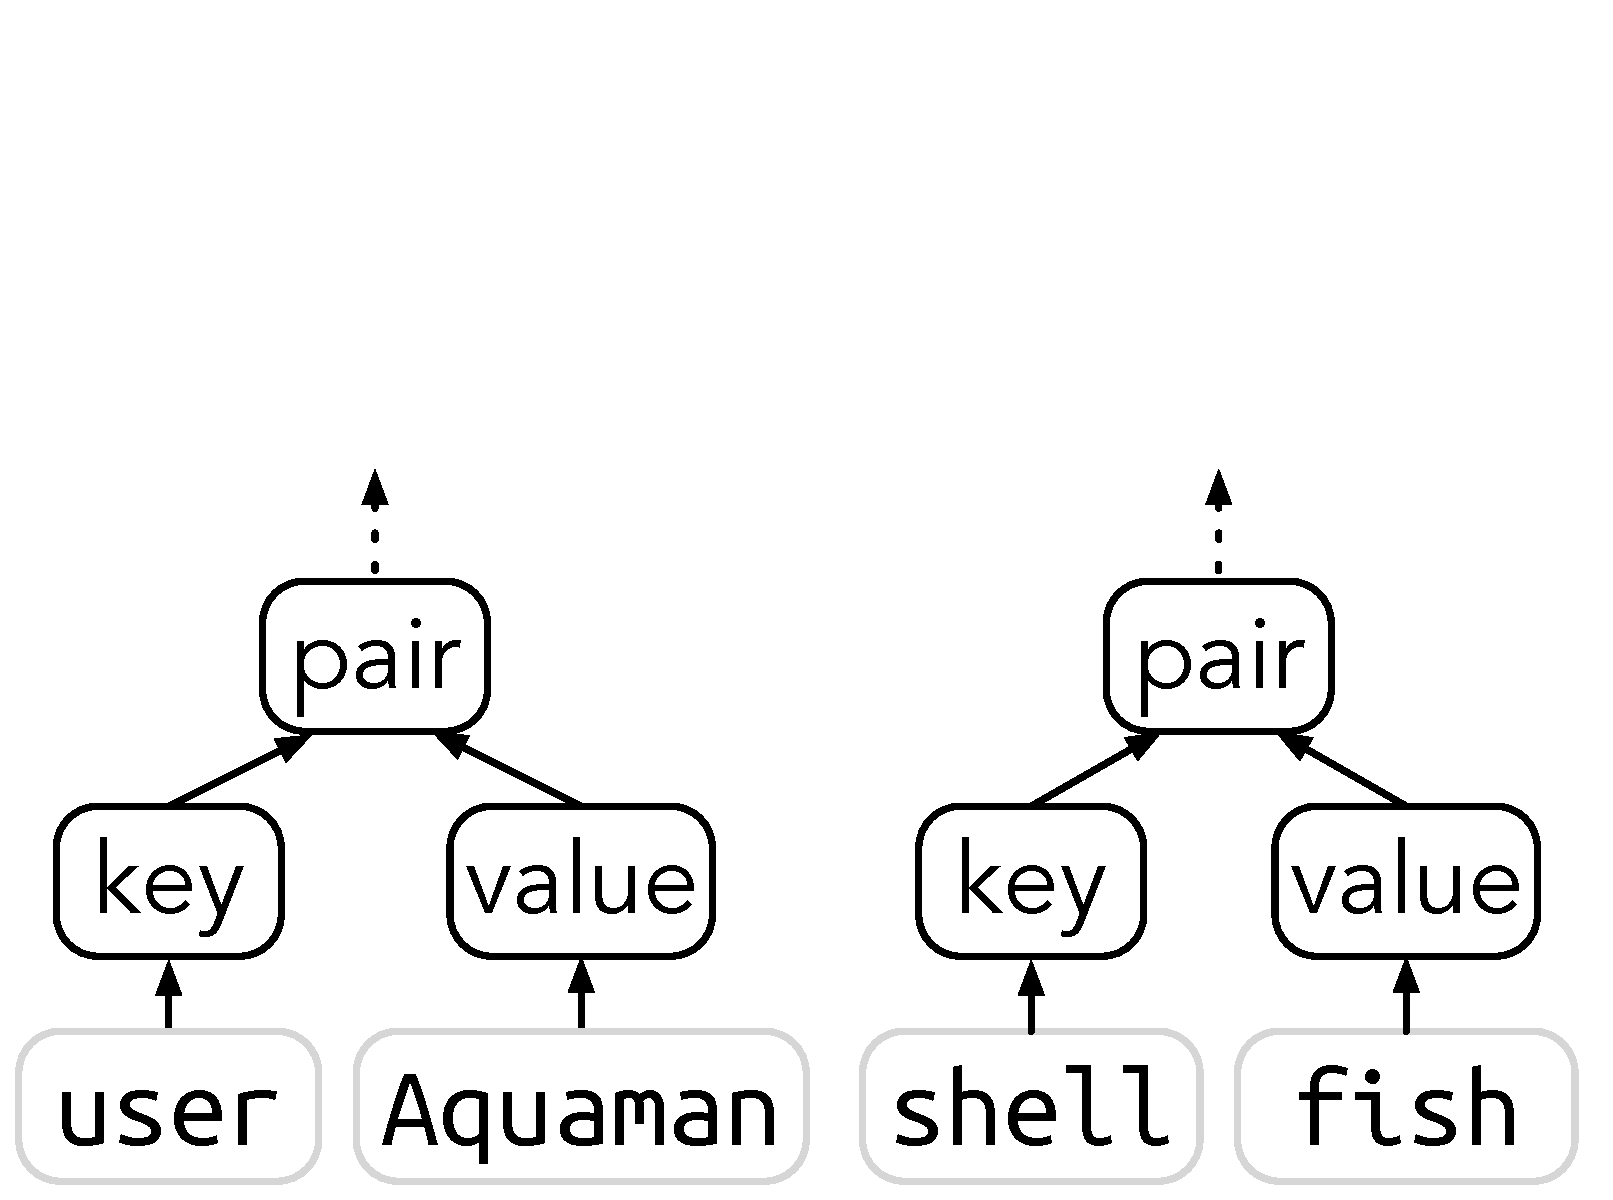
\includegraphics[width=\linewidth]{Bottom-Up}
    \caption{A bottom-up parser recognizes text starting with the terminal symbols.}
  \end{subfigure}
  \caption{Matching in top-down and bottom-up parsers}
\end{figure}

In \emph{top-down parsing} the parser starts with a hypothesis about the structure of the given data. The parser then tries to predict and match parts of the structure, starting from larger parts working its way down to smaller elements.

We can further categorize parsing into \emph{directional} and \emph{non-directional} methods. Directional methods read the input from left to right, while non-directional methods can use an arbitrary order. This implies that directional methods are simpler and faster, but less powerful than their non-directional counterparts. As part of this thesis we only consider directional methods, since they are faster and powerful enough to parse configuration data.

One of the most popular directional top-down methods is \emph{\glstext{LL} parsing}. While this technique is quite old – \citetitle{grune2008parsing} (p. 584) mentions a paper from 1961 belonging to the \glstext{LL} category – it is still actively used and researched. The basic idea behind \glstext{LL} parsing is simple: Begin with the start symbol of the grammar and the first character/\gls{token} of the text. Then predict the next grammar rule, looking at the text to the right of the current position. We can categorize the technique further according to the number of characters/\glspl{token} the parser uses to predict the next rule. If the parser uses one \gls{token} of look-ahead we speak of an \glstext{LL}(1) parser, if it uses k \glspl{token} of lookahead we speak of an \glstext{LL}(k) parser~\cite{rosenkrantz1969properties}.

Two common methods to create an \glstext{LL} parser are:

\begin{enumerate}

  \item Implement the parser code using a set of mutually recursive procedures (recursive descent parser). The code for this is either written by hand or produced by a parser generator such as \GlsShort{ANTLR}~\cite{parr2013recursive}.

  \item Use a parser generator to create a table-based parser.

\end{enumerate}

Examples of popular active projects that use a handwritten recursive descent parser include \href{http://clang.llvm.org}{Clang}~\cite{bendersky2012clang} and \href{http://gcc.gnu.org}{GCC}~\cite{myers2008cparser}. The \href{http://www.antlr.org/about.html}{about page} for \gls{ANTLR} mentions some projects that use its generated recursive descent parsers. The list includes Twitter, wich uses ANTLR for query parsing and parsers for the languages used in the Apache Hadoop projects Hive and Pig~\cite{parr2013definitive}.

Some of the latest research developments in \glstext{LL} parsing include \glstext{LL}(*) parsing~\cite{parr2011ll} and its successor \gls{ALL(*)}~\cite{parr2014adaptive}. Both of these algorithms use dynamic lookahead~\cite[p. 1]{parr2011ll}. While \glstext{LL}(*) parsing uses a static algorithm for rule prediction, ALL(*) analyzes the input at runtime to improve prediction. As consequence of this, parsers that use the \gls{ALL(*)} algorithm will be faster after an initial warm-up phase~\cite[p. 3]{parr2014adaptive}. LL(*) is part of \gls{ANTLR}~3~\cite[p. 3]{parr2014adaptive}, while \gls{ANTLR}~4 uses Adaptive \glstext{LL} parsing.

As we already mentioned before, the other popular parsing technique besides top-down-parsing is \emph{bottom-up parsing}. In bottom-up parsing the parser builds a structure starting with the smallest elements of the grammar (terminals). The parser then combines these elements into larger parts. One of the earliest entries in the \emph{linear bottom-up} parser category is the \glstext{LR}(k) parser~\cite{knuth1965translation}. Just as in \glstext{LL}(k) parsing, k specifies the number of lookahead symbols the parser uses.

\begin{sloppypar}
Unlike \glstext{LL} parsers, \glstext{LR} parsers are usually not created by hand, but generated by a parsing tool such as \href{https://www.gnu.org/software/bison}{Bison} or \href{http://dinosaur.compilertools.net/yacc}{Yacc}. Since \glstext{LR}(k) tables are very large, even for a small numbers of k, the parser tools mentioned before usually generate less powerful but smaller and faster LALR(k)~\cite{deremer1969practical} parsers.
\end{sloppypar}

\glstext{LR}(k) parsers are able to handle more grammars than \glstext{LL}(k) parsers for the same constant k~\cite[section “Lookahead”]{haberman2013ll}. However, \glstext{LR} parsers are still not able to handle ambiguous grammars. For this purpose \citeauthor{lang1974deterministic} describes the Generalized \glstext{LR} (GLR)~\cite{lang1974deterministic} method that is also able to process these types of grammars. GLR parsers are sometimes also called Tomita parsers~\cite{tomita1985efficient} after the author that described the first implementation of a generalized \glstext{LR} parser.

Recent research in the space of directional bottom-up parsing includes improved versions of techniques that are almost as powerful as canonical \glstext{LR}(1). One of the most promising methods is IELR(1)~\cite{denny2008ielr}. The advantage of IELR(1) over LALR(1) is that it handles conflict resolution better. Parser tools such as Bison use conflict resolution to handle non-\glstext{LR} grammars, i.e. grammars that contain rules where the parser is not able to decide what to do next. To handle these types of conflicts the grammar designer manually specifies which decision the parser should take. The current version of the parsing tool Bison supports an experimental version of IELR(1).

Most parsing techniques can be categorized as either top-down or bottom-up. However, some techniques use a combination of both approaches. Others are usually not listed under one of the label top-down or bottom-up, because they provide other features that the designers of these parsers deem more important, or they use features that do not fit well within either of these groups. In the remainder of this section we will discuss some of these techniques.

A method that can be categorized as either top-down technique with bottom-up recognition, or bottom-up technique with a top-down component~\cite[p. 206]{grune2008parsing} is \emph{Earley Parsing}~\cite{earley1970efficient}. Earley parsing is able to handle any context free grammar. This means the technique is as powerful as GLR parsing. This advantage comes at the cost of runtime. While \glstext{LL} parsing and \glstext{LR} parsing run in linear time depending on the length of the input ($O(n)$), Earley Parsing has an upper boundary of $O(n³)$. However, in \citeyear{leo1991general} \citeauthor{leo1991general} showed that an improved version of the algorithm handles most \glstext{LR}(k) grammars in linear time~\cite{kegler2011marpa, leo1991general}. In \citeyear{aycock2002practical} \citeauthor{aycock2002practical} described improvements to the algorithm~\cite{aycock2002practical}. Their version of Earley Parsing boosts the runtime in cases where the grammar contains nullable (empty) grammar rules. Recently \citeauthor{kegler2011marpa} incorporated the changes proposed by \citeauthor{leo1991general}, \citeauthor{aycock2002practical} in \href{http://savage.net.au/Marpa.html}{Marpa}~\cite{kegler2011marpa}.

\begin{figure}
  \centering
    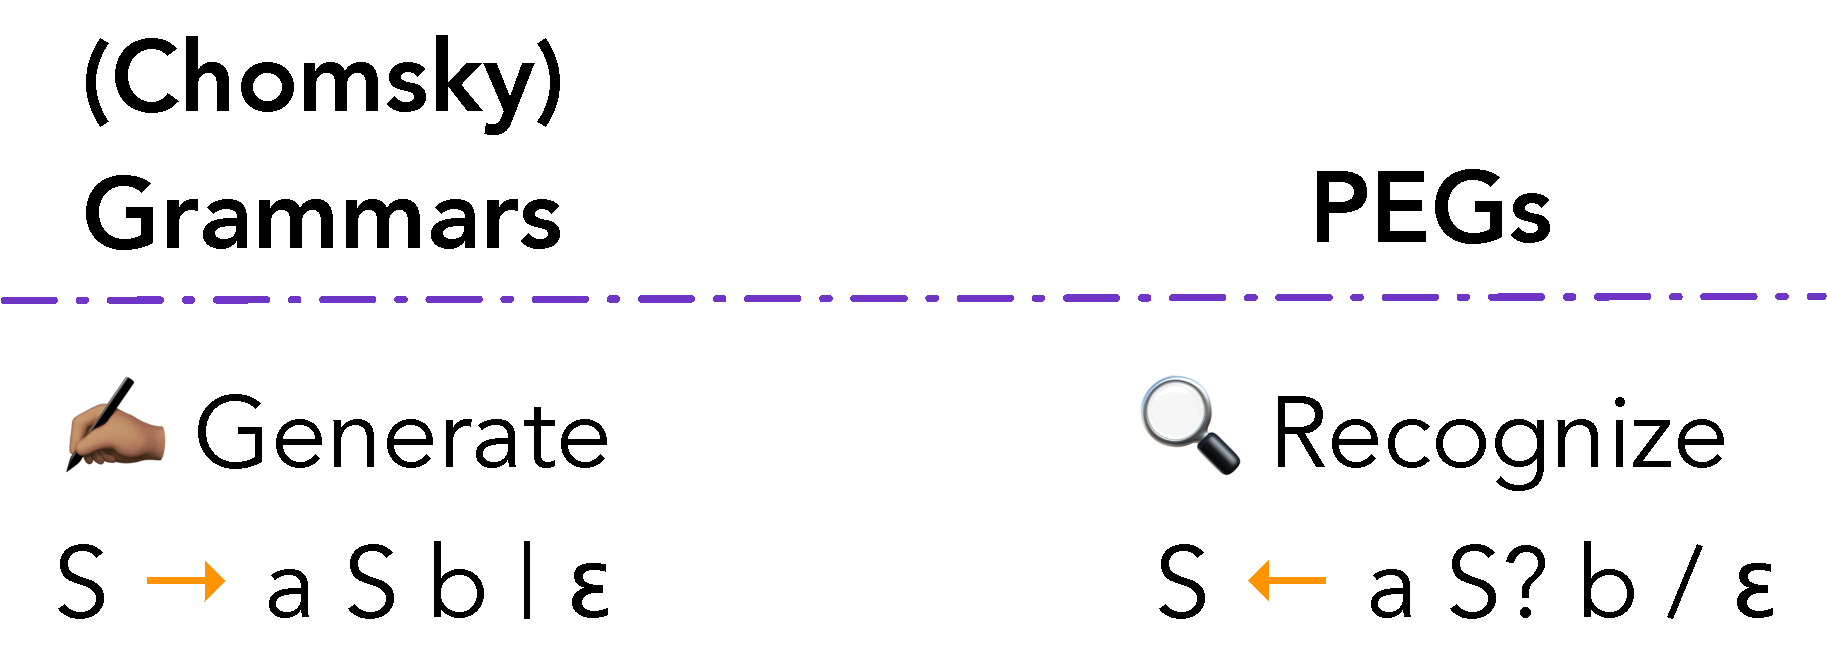
\includegraphics[width=0.45\textwidth]{Chomsky-PEGs}
  \caption{Both the Chomsky grammar on the left and the PEG on the right describe the same language $ \{ aⁿ bⁿ | n ≥ 0 \} $.}
\end{figure}

All the methods we mentioned until now work with a description that is based on a (context-free) Chomsky grammar. These grammars describe a way to \emph{generate} words and sentences of a given language. Another way to specify the structure of a language is to give a description on how to \emph{recognize}~\cite[p. 506]{grune2008parsing} the words and sentences of a language. One popular recognition system are \glspl{PEG}. They were introduced by \citeauthor{ford2004parsing} in the paper \citetitle{ford2004parsing}~\cite{ford2004parsing}. \citeauthor{ford2002packrat} also describes how to write an efficient (top-down) parser that handles these types of grammars in linear time~\cite{ford2002packrat}. This method, called Packrat parsing, uses a specialized version of memoziation~\cite[p. 1]{ford2002packrat} to save intermediate results of the parsing process. We should mention that it is generally not clear, if memoization provides a runtime performance advantage in practice for a certain grammar. In the article~\citetitle{hudak2008dcgs}~\cite{hudak2008dcgs} \citeauthor{hudak2008dcgs} show that not using memoization can decrease the actual runtime of a PEG parser.

Just like Packrat parsing, \emph{combinatory parsing}~\cite{frost1992constructing, hutton1992higher} specifies a method to create recursive descent parsers. As the name suggests, the focus in combinatory parsing is the composability of parsers. The technique is usually used in functional programming languages, such as Haskell. These languages support higher order functions, i.e. functions that take other functions as their parameters~\cite[p. 564]{grune2008parsing}. In combinatory parsing the parser creator typically starts by specifying parsers (functions) for the simplest parts of the grammar (terminals). She or he then goes on to combine these simpler parsers into more powerful parsers for more complex rules (non-terminals). Combinatory parsing has similar problems as other top-down techniques such as \glstext{LL} parsing. One of these problems are left recursive grammar rules, i.e. rules that include references to themselves in the leftmost part of the right-hand side. Recently \citeauthor{frost2007modular} described a method to handle left recursive rules in combinatory parsing efficiently in the article \citetitle{frost2007modular}~\cite{frost2007modular}.

A method that is not a parsing technique per se, but a way to specify conversions of data from a source structure to a target structure and back is \emph{bidirectional programming}~\cite{foster2005combinators, bohannon2006relational}. The specification that allows this conversion is called a lens~\cite{foster2005combinators}.

\begin{figure}[H]
  \centering
    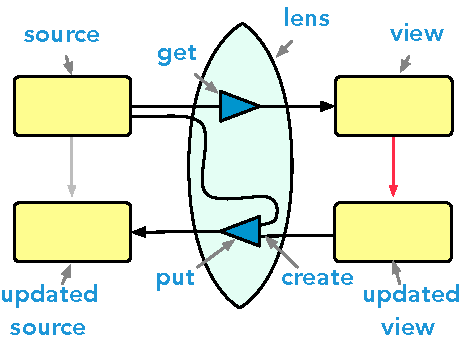
\includegraphics[width=.4\textwidth]{Lens}
  \caption{Lenses provide a way to both parse (get) and write (put) structured data \newline (Source: \href{http://www.seas.upenn.edu/~harmony/manual.pdf}{Boomerang Programmer’s Manual}).}
\end{figure}

A programming language used to specify such lenses is Boomerang~\cite{bohannon2008boomerang}. The research of the Boomerang project lead to the creation of another project that uses lenses to parse configuration data: \href{http://augeas.net}{Augeas}. Augeas converts configuration data into a tree like representation. \citeauthor{berlakovich2016universal} implemented an Augeas plugin for Elektra as part of his Bachelor thesis~\cite{berlakovich2016universal}.

\subsection{Configuration File Parsing}
\label{sec:configuration_file_parsing}

The literature overview in the previous section focused on parsing in general. It is now time to take a look at the current state of configuration file parsing and how it differs from the well know problem of parsing (general purpose) programming languages.

There exists extensive literature about parsing of programming languages and compiler design. The topic is even part of famous computer science books such as \citetitle{ullman1977principles}~\cite{ullman1977principles} and \citetitle{aho2006compilers}~\cite{aho2006compilers}, commonly also know as “Dragon” books~\cite{parr2009language}, named after the Dragon (waiting to be slain) on their covers.

While parsing and compiling computer languages is seen as “slaying a Dragon”, configuration file parsing is arguably a much simpler task. The reason for this is that the purpose of configuration languages, usually only specifying data, is a subset of the purpose of programming language, which also manipulate data. This superset feature of programming language makes them sometimes also interesting for the purpose of storing configuration data~\cite{balmer2013lua}. Since configuration data is used by many programs that usually do not ship with, or require an interpreter or compiler, most configuration files do not use the syntax of a general purpose programming language. These “data only” configuration file formats can be classified roughly into three categories.

\begin{description}
  \item[Custom configuration file formats] specify data for a specific application. Examples are the \href{https://en.wikipedia.org/wiki/Fstab}{\code{fstab}} file used by the Unix program \sh{mount} or the \href{https://en.wikipedia.org/wiki/https://en.wikipedia.org/wiki/Hosts_file}{\code{hosts}} file used for name resolution.

  \item[General purpose configuration formats] such as \href{https://en.wikipedia.org/wiki/INI_file}{INI}, and the \href{https://en.wikipedia.org/wiki/Property_list}{Property list} file format are used mainly to store configuration data of many different applications.

  \item[Serialization formats] such as \gls{JSON}, \gls{YAML}, and \gls{XML}, store all kinds of data, not only limited to configuration purposes.
\end{description}

\begin{figure}[H]
  \centering
  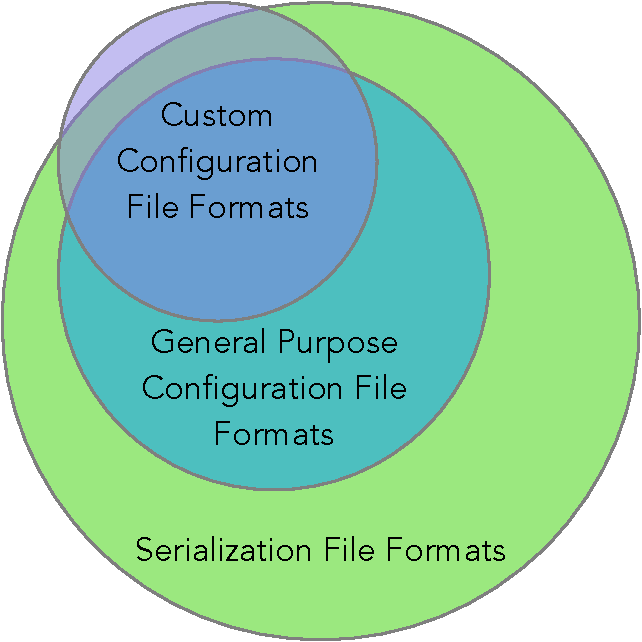
\includegraphics[width=.45\textwidth]{ConfigurationFileFormats}
  \caption{The Venn diagramm above shows an overview of the overall expressiveness of the formats usually used for configuration data. Please note, that the size of the circles \emph{does not} show the level of expressiveness of a certain category of file formats, i.e. a circle twice as large does not represent twice the level of expressiveness.}
\end{figure}

In general we can use serialization formats, to specify the same data as we can using general purpose configuration languages. For example, in macOS Property lists can be stored using \glstext{JSON} or \glstext{XML} on disk. The same is not true for custom configuration formats, which are often very simple, but can sometimes also use programming language code. Popular examples for this are the configuration files of shells, such as \code{bash}, \code{fish} and \code{zsh}. These shells use the same syntax for programming and configuration data.

We already said that most configuration file formats do not use the syntax of general purpose programming languages, but rather syntax only able to specify and \emph{not} to modify data. The simplicity of some of these languages often means that parsing code for them is not written by an expert. Especially for simple custom configuration file formats, the same person that implements a program often also implements the parser for its configuration file format. This can result in configuration code that integrates tightly into a program, decreasing the extensibility of the application. Other problems of parsers not written by experts include: bad or no error message support, no support for error recovery, and insufficient support for different file format encodings.

Some of these problems can be solved using a configuration file library that is available for most of the more popular general file formats. Such a library takes care of the parsing, loosening the integration of an application and its configuration code. Some problems of theses libraries are that they

\begin{itemize}
  \item often do not consider order, and
  \item almost always throw away comments
\end{itemize}

when they write back data into a configuration file. This is a problems, since for example, comments in configuration files can be very helpful in averting misconfiguration.

A configuration library that keeps the order of entries and comments intact is Augeas~\cite{lutterkort2008augeas, berlakovich2016universal}. As we already wrote in the previous section Augeas uses so-called lenses to both parse and write back configuration. The problem of lenses is that they only support regular languages~\cite{chomsky1959certain} properly. For example, as we found out during the development of the parsing code for the thesis, the \href{https://github.com/hercules-team/augeas/blob/d555a995a06ac81cab62d016d6eaff8a7ba64a2e/lenses/yaml.aug}{YAML lens} of Augeas only supports mapping data with a nesting level of two.

Compared to Augeas, Elektra~\cite{raab2010modular, raab2017context}, with its plugin-based parsing system also supports context free and even context sensitive configuration languages. This is the case, since Elektra can use a general purpose programming language to parse code. Using metadata Elektra is also able to store the content of comments and keep the order of configuration data intact, when writing data back. The code for this has to be implemented in the plugin itself, which can become problematic. For example, while Elektra’s \href{https://github.com/ElektraInitiative/libelektra/tree/3e6e0254a54d3ad9642091550ce9c560d8cf38dd/src/plugins/ini}{INI plugin} preserves comments and the order of entries, its code is also quite complicated and error-prone. As we already stated in “\nameref{sec:aim_of_the_work}” we want to improve this situation using state of the art parsing techniques for our YAML subset plugins.

\subsection{Error Handling}
\label{sec:error_handling}

The usual goal in parsing is the processing of grammatically correct input. However, since editing configuration data is often done by hand, there is always a possibility of erroneous input. A method to inform the user about such errors is essential. As pointed out by Terence \citeauthor{parr2013definitive} in \citetitle{parr2013definitive}~\cite[p. 151]{parr2013definitive} we also need to inform the user about the reason for an error:

\begin{quote}
  In other words, a parser that responds with “Eh?” and bails out upon the first syntax error isn’t very useful for us during development or for our users during deployment.
\end{quote}

The process of reacting to errors is called \emph{error handling}. Error handling can be grouped into four dependent stages~\cite{ruefenacht2016error, pottier2016reachability}:

\begin{enumerate}
  \item error detection,
  \item error diagnosis,
  \item error recovery, and
  \item error correction
\end{enumerate}

. We are mainly interested in the first three items, since error correction is generally not possible without the possibility of fixing errors incorrectly.

\emph{Error reporting} is the results of

\begin{itemize}
  \item detecting that input is incorrect (error detection),
  \item finding what part of the input was incorrect (error diagnosis), and
  \item trying to resume the parsing process in case of errors (error recovery).
\end{itemize}

The current state of error reporting capabilities depend strongly on the parsing technique.

In general, top-down recursive descent parsers \emph{without backtracking}, especially those written by hand, are able to produce good error messages. The reason for this is that such parsers have information about the higher level grammar rules that matched until the error point. While the error messages produced by recursive descent parsers can be good, writing error logic by hand makes the code more complicated. If we want to react to multiple errors in a configuration file we also need to implement error recovery, which can be “tedious and easy to screw up”~\cite[p. 160]{parr2013definitive}. \glstext{ANTLR} produces parsers that integrate techniques such as \gls{token} deletion, \gls{token} insertion, and resynchronization to produce parsers that provide “a good error reporting facility and a sophisticated error recovery strategy for free” according to its main author~\cite{parr2013definitive}.

Bottom-up parsers produced by a tool such as Bison are not suited to provide good error messages~\cite{jeffery2003generating}. Error recovery in Bison produced parsers even requires changes to the grammar~\cite{donnelly2019bison}. There exists promising research work to improve the current situation. In \citetitle{jeffery2003generating}~\cite{jeffery2003generating}  \citeauthor{jeffery2003generating} shows how his tool merr can help a user to specify error messages based on example input in a C based parser produced by \glstext{Yacc} or Bison. \citeauthor{jeffery2003generating}’s semi-automated approach is based on error states of the parser and improves on the previous technique used in the Icon programming language, where developers manually modified the source code produced by a custom version of \glstext{Yacc}. Since  \citeauthor{jeffery2003generating}’s work looks promising, another similar approach was also used in the old Bison parser\footnote{The developers of Go switched to a hand-written parser written in Go in 2016~\cite{pike2017reddit, go2016release}.} for the programming language Go~\cite{cox2010errors}. Recently \citeauthor{pottier2016reachability}~\cite{pottier2016reachability} extended \citeauthor{jeffery2003generating}’s work and added example based error reporting in the \glstext{LR} parsers of the CompCert C compiler~\cite{kaestner2018compcert}. In \citetitle{pottier2016reachability} \citeauthor{pottier2016reachability}~\cite{pottier2016reachability} writes that he thinks that “the quality of CompCert’s diagnostic messages is now on par with that of \texttt{clang} and \texttt{gcc}”.

For now we only talked about the error capabilities of deterministic parsers – such as \glstext{LL} and \glstext{LR} parser – i.e. parser that do not back up. These parsers read the input deterministically from left to right. They therefore report the first position, where the parsed input is not part of the language described by the grammar anymore. This behavior is also known as (longest) correct/viable prefix property~\cite{sippu1990parsing, ruefenacht2016error, maidl2016labeled, pottier2016reachability}. Parsers with backtracking, such as recursive descent parsers \emph{with backtracking}, \glstext{PEG} parsers and the closely related combinatory parsers usually do not have this property. While backtracking makes these parsers more powerful, the quality of error messages suffer. The problem is that backtracking can occur both because of a valid choice in the grammar or because of an error in the input.

There has been research to improve the situation, especially in \glstext{PEG} parsers. In his master thesis~\cite{ford2002packrat} \citeauthor{ford2002packrat} already describes one option to produce meaningful error messages. His parser records all parsing results and uses the one that matched the farthest to the right in the input for error messages. In \citetitle{maidl2016labeled}~\cite{maidl2016labeled} \citeauthor{maidl2016labeled} show that this error strategy can also be added to every \glstext{PEG} library that supports semantic actions. They also introduce a form of error reporting, inspired by the excepting handling mechanism of programming languages, based on grammar annotations called labeled failures~\cite{maidl2016labeled}.

\section{Elektra}

In this section we describe some of the concepts of Elektra, the software that provides the common storage facility for our \glstext{YAML} parsers, further. Elektra is a framework that stores data in a \emph{global hierarchical key-value database}.

\subsection{\cc{Key}}

\begin{figure}
  \centering
    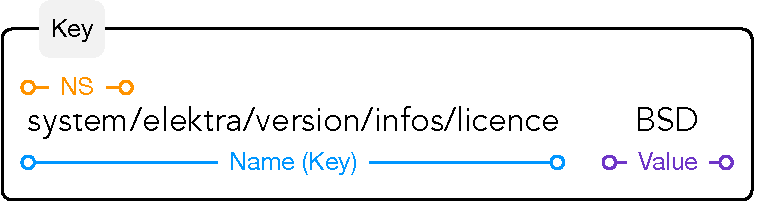
\includegraphics[width=.6\textwidth]{Key.pdf}
  \caption{In Elektra a \cc{Key} stores a single \textcolor{Aqua}{key}-\textcolor{Purple3}{value} pair. The first part of the name specifies the \textcolor{orange}{namespace (\glstext{NS})}.}
  \label{fig:key}
\end{figure}

The most basic entity in Elektra is the \cc{Key} structure. A concrete instance of a \cc{Key} contains at least one non-empty attribute, which is the \emph{name} of the \cc{Key}. In the remainder of the thesis we will also often use the term \emph{key} - please notice the non-gray background – to refer to the name of a \cc{Key}.

Besides the name an instance of a \cc{Key} usually also stores a value. Figure~\ref{fig:key} shows an example \cc{Key} with the \textcolor{Aqua}{name} \code{system/elektra/version/infos/licence} and the \textcolor{Purple3}{value} \code{BSD}.

Since Elektra stores data in a hierarchical database, a key consists of parts – separated by \code{/} – that determine the location in the database. The key in Figure~\ref{fig:key} consists of 5 parts. The first part \code{system} is the \textcolor{orange}{namespace (\glstext{NS})} of the key. Elektra uses namespaces to specify context dependent data. For example, user specific data is stored under the namespace \code{user}. Elektra uses 5 namespaces to separate data:

\begin{itemize}[style=multiline, leftmargin=1.8cm]
  \item [\code{system}] specifies data values for the whole system,
  \item [\code{user}] contains data for the current user,
  \item [\code{dir}] stores data for the current directory,
  \item [\code{spec}] contains specification of other keys, and
  \item [\code{proc}] stores in-memory data.
\end{itemize}

We can use a so-called \emph{cascading} key to select the most appropriate namespace. A cascading key does not start with a namespace but rather with a leading slash. Let us look at an example. We assume our database contains the keys:

\begin{itemize}
  \item \code{system/key}, and
  \item \code{user/key}.
\end{itemize}

If a non-superuser requests the cascading key \code{/key}, then Elektra will select \code{user/key}. If the database also contains a key \code{dir/key} for the current working directory, then Elektra will select this key instead.

\subsection{\cc{KeySet}}
\label{sec:keyset}

As we already saw in the example before, usually we store not only one, but multiple key-value pairs in the database. For this purpose Elektra provides the structure \cc{KeySet}. A \cc{KeySet} contains a set of \cc{Key} objects. The name of each \cc{Key} has to be different. If we add a new \cc{Key} with an already existing name to the \cc{KeySet}, then Elektra will just overwrite the old \cc{Key} with the same name.

\begin{figure}
  \centering
    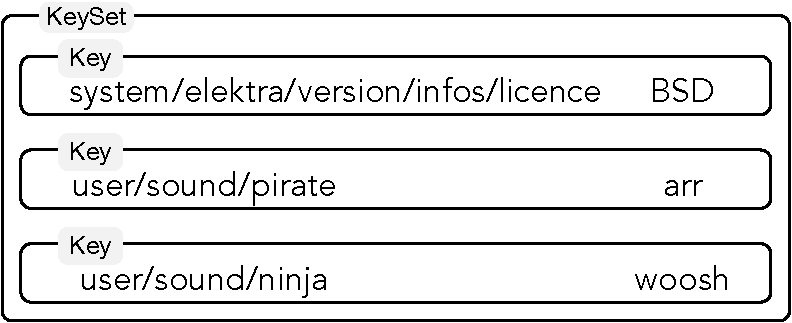
\includegraphics[width=.6\textwidth]{KeySet}
  \caption{Elektra uses \cc{KeySet} structures to save multiple key-value pairs}
  \label{fig:keyset}
\end{figure}

A \cc{KeySet} allows us to structure data in a fashion similar to a map (a.k.a. hash, map, hashmap, dictionary). Maps are an important data structure, especially in high level programming languages like \href{https://www.python.org}{Python} or \href{https://www.ruby-lang.org}{Ruby}. Let us look at an example. We take the last three \cc{Key} objects in Figure~\ref{fig:keyset}, remove the namespace and translate the data to a Python dictionary:

\begin{pythoncode}
  sound = {'pirate': 'arr', 'ninja': 'woosh'}
\end{pythoncode}

. We see that a value in a \cc{KeySet} also maps to a value in the dictionary, while the last part of the key (name) maps to the key in the dictionary.

Apart from the map, another important data structure is the array. Elektra also supports arrays. For that purpose Elektra adds the character \code{\#}, and the index to array elements. For example, the following Python list:

\begin{pythoncode}
  characters = ['pirate', 'ninja']
\end{pythoncode}

would translate to the \code{KeySet} shown in Figure~\ref{fig:array}.

\begin{figure}
  \centering
    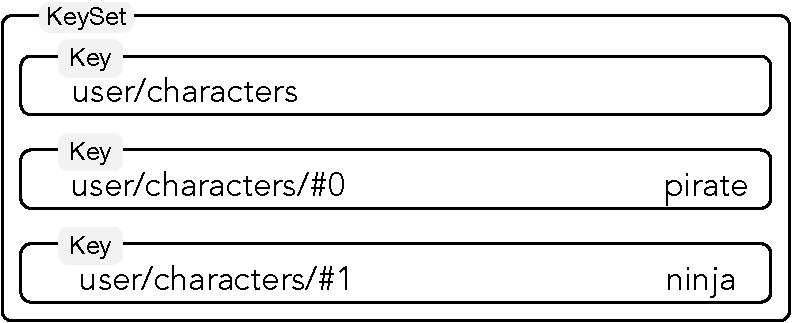
\includegraphics[width=.6\textwidth]{Array}
  \caption{Elektra uses the character \code{\#} to mark array elements}
  \label{fig:array}
\end{figure}

Since Elektra orders a \code{KeySet} alphabetically a \cc{Key} with name \code{\#10} would appear before a \cc{Key} with name \code{\#2}. To fix that problem Elektra adds underscores to keys with larger indizes. For example, the 11th element of an array ends with the name \code{\#\_10}.

One important difference between Python’s list type and Elektra’s array type is that arrays do not need to be continuous. For example, it is possible for an Elektra array to only contain elements with the names \code{\#1} and \code{\#3}, while \cc{Key} entries with name \code{\#0} and \code{\#2} are missing.

Elektra also uses the \cc{KeySet} structure to add \emph{metadata} to single keys. For this purpose each \cc{Key} may store a \cc{KeySet} containing simple key-value pairs. Figure~\ref{fig:metadata} shows an example \cc{Key} containing two meta keys \code{comment} and \code{check/type}.

\begin{figure}
  \centering
    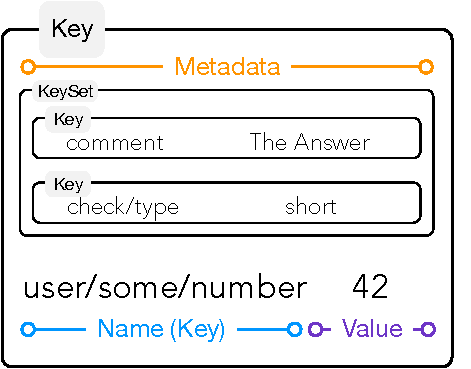
\includegraphics[width=.4\textwidth]{Metadata}
  \caption{Elektra uses a \cc{KeySet} to save metadata for a \cc{Key}.}
  \label{fig:metadata}
\end{figure}

\FloatBarrier
\subsection{Plugins}
\label{sec:plugins}

Apart from basic features, most of Elektra’s functionality is realized as \emph{plugin}. This has the advantage, that Elektra’s core can stay minimal only requiring \href{https://en.wikipedia.org/wiki/C99}{C99}, while plugins are able to implement and use OS specific features.

Many different \href{https://www.libelektra.org/plugins}{plugin categories} exist. Elektra needs at least one resolver and one storage plugin. The resolver plugin handles filenames and replaces files on disk. Storage plugins, on the other hand, parse configuration files and convert read data to a \cc{KeySet}. They are also responsible for writing a modified \cc{KeySet} back to a given file.

In this thesis we are mostly interested in storage plugins. However, we will also use other plugins to implement common functionality for our \glstext{YAML} storage plugins. For this purpose we use the plugin interface of Elektra to pass key sets between plugins.

The order in which Elektra calls a certain plugin is specified via the \emph{contract} of the plugin. For example, a typical storage plugin will use the positions \code{getstorage} and \code{setstorage}. Plugins at the position \code{getstorage} will be called when Elektra tries to read a configuration file, while Elektra calls \code{setstorage} plugins when it is time to write a \cc{KeySet} back to a file. A plugin that wants to further process data will usually use the position \code{postgetstorage} right after \code{getstorage}, and \code{presetstorage} the position before \code{setstorage}.

\begin{figure}
  \centering
    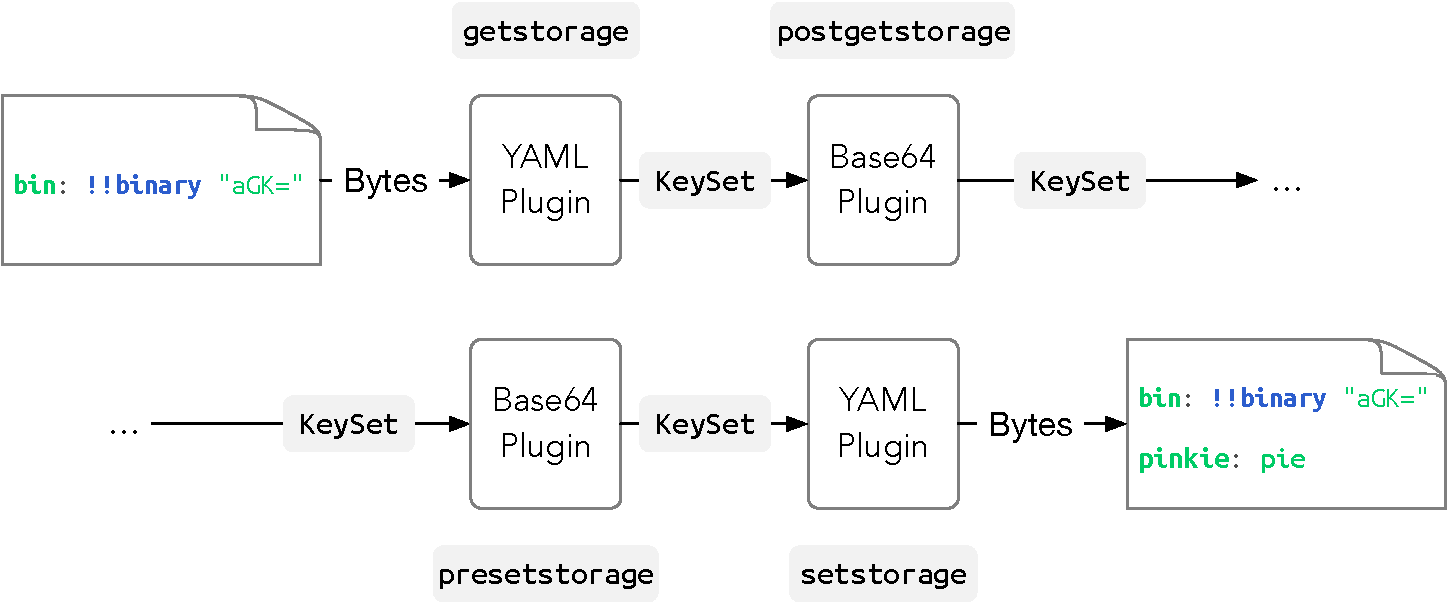
\includegraphics[width=.9\textwidth]{Plugins}
  \caption{Elektra uses multiple plugins to process data.}
  \label{fig:plugins}
\end{figure}

Figure~\ref{fig:plugins} shows a example, where Elektra uses a \glstext{YAML} plugin to read and write data, while a Base64 plugin (see also section “\nameref{sec:base64}”) encodes and decodes binary values. Such a combination of multiple plugins working together is called a \emph{backend}.

In Elektra we \emph{mount} a backend at a certain position of the key-value database. For example, if we mount the backend described above at \code{user/yaml}, then the \glstext{YAML} plugin is responsible for storing and retrieving values below this mountpoint. If we want to save a new \cc{Key} with the name \code{user/yaml/pinkie} and the value \code{pie}, then Elektra

\begin{enumerate}
  \item uses the \glstext{YAML} plugin to convert the current \glstext{YAML} configuration file to a \cc{KeySet},
  \item decodes every binary \cc{Key} with the Base64 plugin,
  \item adds \code{user/yaml/pinkie} to the \cc{KeySet},
  \item encodes every binary \cc{Key} with the Base64 plugin, and
  \item then stores the result to the configuration file using the \glstext{YAML} plugin.
\end{enumerate}

\section{Related Work}

Most of the parser comparison related papers evaluate some form of new parser engine or parser generator against existing parsers or libraries. A recent example of this type of paper is \citetitle{json2019geoff}~\cite{json2019geoff}. In this paper \citeauthor{json2019geoff} use \gls{SIMD} instructions to accelerate the parsing of \gls{JSON} data. In the “Experiments” section of this paper the authors compare their implementation with other JSON parsers, first only using the pure parsing speed, meaning that they ignore the different output of the tested parsers. They also provide a comparison where they show how fast the tested parser are able to find the same data in one of the converted documents from their data set.

While parsing one file format using a specialized parser provides information about how fast we are able to convert certain file formats, this kind of optimization can require substantial manual work. For the plethora of different configuration file formats, it is usually not possible to handcraft parser by hand. Even if it would be possible, some parser need to store information that others do not (e.g. comments), making the process of creating a parser that handles all these tasks by hand even harder. To fix this problem we can generate code for the parser.

There are some papers that compare parser generators themselves. For example, in \citetitle{chen2011full}~\cite{chen2011full} \citeauthor{chen2011full} compare the table size and the time to generate parser code for the tools Hyacc, Menhir, MSTA and Bison. This paper does not evaluate the execution speed, error messages or other important criteria of the generated parsers.

In \citetitle{flodin2014packrat}~\cite{flodin2014packrat} \citeauthor{flodin2014packrat} compares a modified version of the PEG parser Treetop – adapted to produce C++ code – called Hilltop, and \gls{Yacc}. He measures both the execution speed and the heap memory usage of the generated parsers for two different grammars. He does not compare other important criteria, such as the generated error messages, mainly because the parsers generated by Treetop only print information about the last successful production.
